% This is "sig-alternate.tex" V1.3 OCTOBER 2002
% This file should be compiled with V1.6 of "sig-alternate.cls" OCTOBER 2002
%
% This example file demonstrates the use of the 'sig-alternate.cls'
% V1.6 LaTeX2e document class file. It is for those submitting
% articles to ACM Conference Proceedings WHO DO NOT WISH TO
% STRICTLY ADHERE TO THE SIGS (PUBS-BOARD-ENDORSED) STYLE.
% The 'sig-alternate.cls' file will produce a similar-looking,
% albeit, 'tighter' paper resulting in, invariably, fewer pages.
%
% ----------------------------------------------------------------------------------------------------------------
% This .tex file (and associated .cls V1.6) produces:
%       1) The Permission Statement
%       2) The Conference (location) Info information
%       3) The Copyright Line with ACM data
%       4) NO page numbers
%
% as against the acm_proc_article-sp.cls file which
% DOES NOT produce 1) thru' 3) above.
%
% Using 'sig-alternate.cls' you have control, however, from within
% the source .tex file, over both the CopyrightYear
% (defaulted to 2002) and the ACM Copyright Data
% (defaulted to X-XXXXX-XX-X/XX/XX).
% e.g.
% \CopyrightYear{2003} will cause 2002 to appear in the copyright line.
% \crdata{0-12345-67-8/90/12} will cause 0-12345-67-8/90/12 to appear in the copyright line.
%
% ---------------------------------------------------------------------------------------------------------------
% This .tex source is an example which *does* use
% the .bib file (from which the .bbl file % is produced).
% REMEMBER HOWEVER: After having produced the .bbl file,
% and prior to final submission, you *NEED* to 'insert'
% your .bbl file into your source .tex file so as to provide
% ONE 'self-contained' source file.
%
% ================= IF YOU HAVE QUESTIONS =======================
% Questions regarding the SIGS styles, SIGS policies and
% procedures, Conferences etc. should be sent to
% Adrienne Griscti (griscti@acm.org)
%
% Technical questions _only_ to
% Gerald Murray (murray@acm.org)
% ===============================================================
%
% For tracking purposes - this is V1.3 - OCTOBER 2002

\documentclass{sig-alternate}
\usepackage{graphics}

\begin{document}
%
% --- Author Metadata here ---
\conferenceinfo{DAC}{'10 Anaheim, CA, USA}
%\CopyrightYear{2001} % Allows default copyright year (2000) to be over-ridden - IF NEED BE.
%\crdata{0-12345-67-8/90/01}  % Allows default copyright data (0-89791-88-6/97/05) to be over-ridden - IF NEED BE.
% --- End of Author Metadata ---

\title{RICH-IP: An Interactive System for Configurable High-Level IP Synthesis}
%\subtitle{[Extended Abstract]
%\titlenote{A full version of this paper is available as
%\textit{Author's Guide to Preparing ACM SIG Proceedings Using
%\LaTeX$2_\epsilon$\ and BibTeX} at
%\texttt{www.acm.org/eaddress.htm}}}
%
% You need the command \numberofauthors to handle the "boxing"
% and alignment of the authors under the title, and to add
% a section for authors number 4 through n.
%
% Up to the first three authors are aligned under the title;
% use the \alignauthor commands below to handle those names
% and affiliations. Add names, affiliations, addresses for
% additional authors as the argument to \additionalauthors;
% these will be set for you without further effort on your
% part as the last section in the body of your article BEFORE
% References or any Appendices.

%\numberofauthors{2}
%%
%% You can go ahead and credit authors number 4+ here;
%% their names will appear in a section called
%% "Additional Authors" just before the Appendices
%% (if there are any) or Bibliography (if there
%% aren't)
%
%% Put no more than the first THREE authors in the \author command
%\author{
%%
%% The command \alignauthor (no curly braces needed) should
%% precede each author name, affiliation/snail-mail address and
%% e-mail address. Additionally, tag each line of
%% affiliation/address with \affaddr, and tag the
%%% e-mail address with \email.
%\alignauthor Yibo Fan\\
%       \affaddr{Department of Electronic Engineering}\\
%       \affaddr{Shanghai Jiao Tong University}\\
%       \affaddr{Shanghai, China}\\
%       \email{yibo.fan@gmail.com}
%\alignauthor Kenny Q. Zhu\\
%       \affaddr{Department of Computer Science \& Engineering}\\
%       \affaddr{Shanghai Jiao Tong University}\\
%       \affaddr{Shanghai, China}\\
%       \email{kzhu@cs.sjtu.edu.cn}
%}
%\additionalauthors{Additional authors: John Smith (The Th{\o}rv\"{a}ld Group,
%email: {\texttt{jsmith@affiliation.org}}) and Julius P.~Kumquat
%(The Kumquat Consortium, email: {\texttt{jpkumquat@consortium.net}}).}
%\date{30 July 1999}
\maketitle
%A category including the fourth, optional field follows...
\category{B.6.3}{Logic Design}{Design Aids}[Automatic synthesis, Hardware description languages]

\terms{Design, Languages}

\keywords{IP design, Hardware synthesis}
\section{Introduction}

Protein$-$protein interactions (PPIs) are of central importance for the majority of biological functions, such as signal transduction, metabolic pathways, molecular dynamics, and protein networks\cite{Hoffmann.Krallinger.ea:2005}, for they serve as the most fundamental building blocks of the entire interacademic systems of any organisms. Collecting data on pairwise interaction relationships is essential for multiple purpose, including identification of modules with certain functionality\cite{Spirin.Mirny.03}, mapping diseases to dominated genes\cite{Ideker.Sharan.08}, and after all, understanding wholistic metabolic/genetic networks from a system biology perspective.

A lot of databases have been built to store protein and genetic interactions from major model organism species and are available in various standardized formats, such as MINT\cite{Zanzoni.Montecchi-Palazzi.ea:2002}, BIND\cite{Bader.ea:2003}, BIOGRID\cite{DBLP:journals/nar/StarkBRBBT06}, etc. Among those mainstream databases, the data largely rely on voluntary reports by scientists or researchers, besides, comprehensive curation efforts become indispensable for the sake of accuracy. However, the amount of biology-related literatures with respect to protein interactions grows explosively and thus make it either impossible or impractical to manually detect PPI information anymore.

Considering huge amount of PPI information with great wealth hidden in published papers, in recent years, numerous mining techniques have been proposed that aim to extract PPI information automatically from free text, especially machine learning, information retrieval, and natural language processing\cite{DBLP:journals/bib/WinnenburgWPDS08}.These approaches can be roughly categorized into three classes: co$-$occurrence, rule$-$based, and machine learning. 

Co$-$occurrence is the approach with most simplicity and naivete. Just as its name implies, this method intends to find out pairs of proteins that co-occur in the same context. The scope of "same context" ranges from phrase, sentence, paragraph to whole abstract, even document. The underlying assumption is that whenever two proteins are mentioned together by authors, chances are high that there is some kind of relationship between them. However, however, in-context closeness even semantic relation does not necessarily represent actual biological interaction. As a consequence, a large fraction of candidate pairs are mismatched inevitably, causing a high recall but low precision.

The second approach is rule-based extraction, in other words, pattern matching. There are many types of rules, most of them concern natural language processing (NLP). One way is to specify hand-crafted regular expressions before hand, which mostly lean on language usage preference. Besides, by using full or partial (shallow) parsing strategies, more information would be acquired, such as part-of-speech taggers, local dependencies between syntactic components, context-free grammar\cite{DBLP:journals/bioinformatics/TemkinG03}, and full sentence structure. Compared to co$-$occurrence, rule-based approach enjoy better precision but much lower recall. In addition, since the rules are usually derived from training data, that is to say, the improper choice of training data would be significantly lethal, therefore quality of extraction is invariably instable and may not applicable to other data.

The third and most commonly used approach use machine learning techniques, in this case, the task to extract protein$-$protein interactions turns out to be a binary classification problem. Each protein pairs are represented along with a set of features, which is associated with their context, then a well$-$defined classifier gives the answer whether the candidate protein pairs is classified to be qualified PPI. (TO BE FURTHER FILLED!!!)

In this paper, we introduce a general bootstrapping framework for Protein$-$protein interaction extraction from natural text.Our method differs from most of the previous works in three aspects:

(1)The extraction process is driven by only tiny fraction of training data, which are regarded as seed data. In each round, it would derive reliable patterns automatically from seed data, then extract more positive PPI pairs consequently, what's more, the seed data would be augmented by the newly extracted results with high confidence.

(2)multiple graph kernel. 

(3)various evaluation.




\section{The Main Idea}

\begin{figure}[t]
\begin{center}
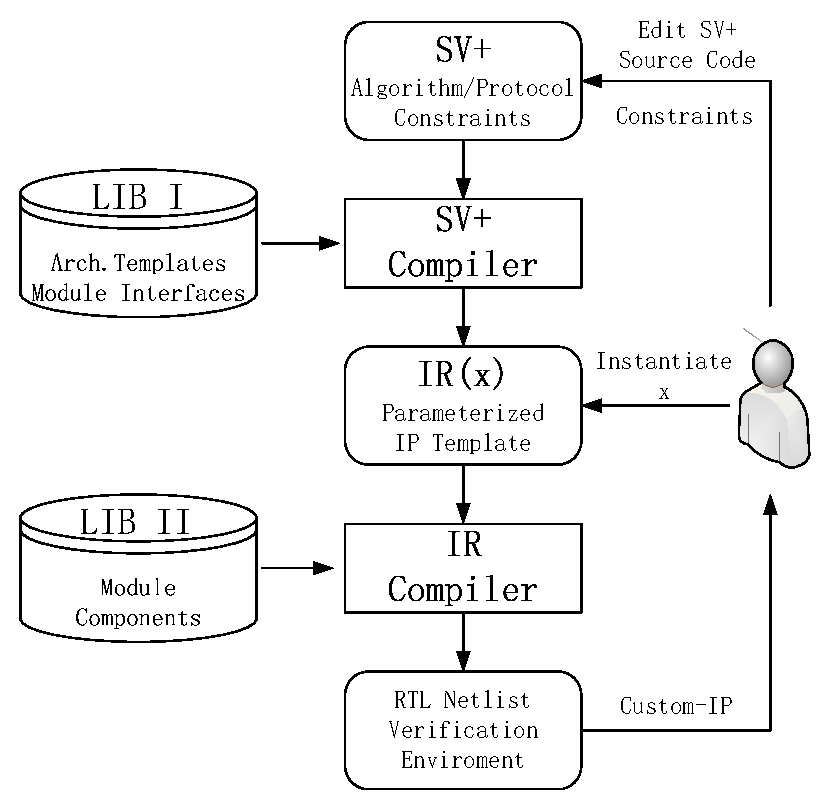
\epsfig{file=arch.eps, width=0.7\columnwidth}
\caption{The architecture}\label{fig-idea}
\end{center}
\end{figure}

%\begin{figure}[t]
%\begin{center}
%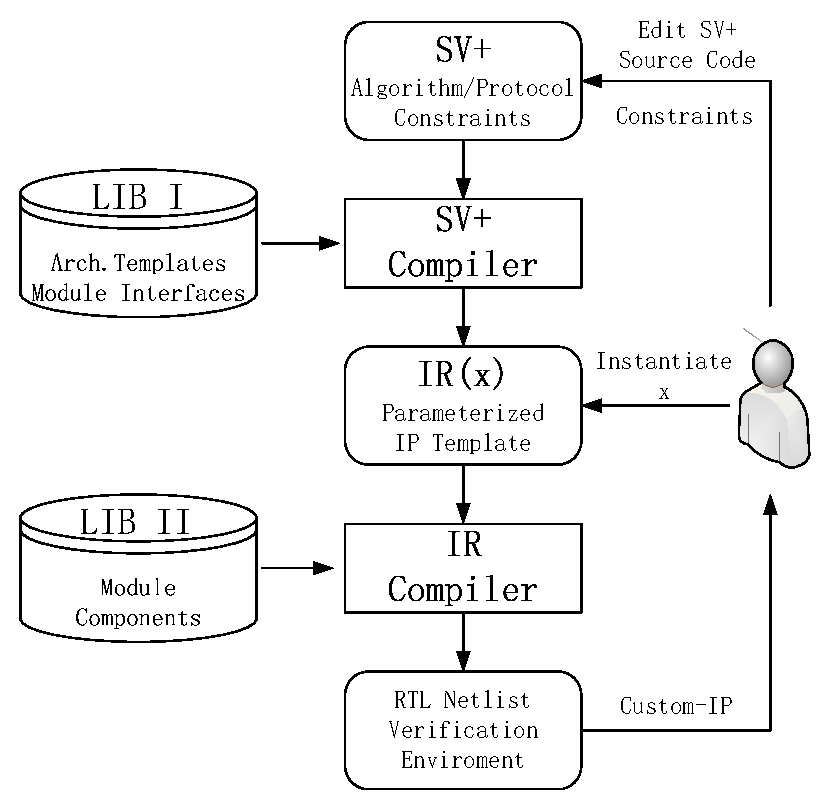
\includegraphics{arch.gif}
%\caption{The architecture}\label{fig-idea}
%\end{figure}


Figure \ref{fig-idea} depicts the architecture of the proposed the RICH system. 
The IP designer describes the algorithm, IP interfaces as well as constraints in SV+, 
a language extension to SystemVerilog. 
The constrains define the physical properties of IP, such as maximum frequency, area cost, or minimum throughput.
The SV+ code then gets preprocessed by an SV+ preprocessor.
This is a coarse-grained IP generation step in which the preprocessor searches
through the {\em template library} to locate most suitable hardware templates that satisfies the
IP constraints and module interfaces. The result of the preprocessing is a parameterized 
intermediate representation of the algorithm, IR($x$),  where $x$ is a set of variable parameters. 
At this point, the designer instantiate these variables using a configuration file. 
Finally, in a fine-grained IP generation step, the fully
instantiated IR is compiled into the RTL and verification environment with
the help of the module library. The end result of the entire flow is a custom IP core, 
and it is passed to the designer for verification.
In case the generated custom IP core does not match the specification, 
the designer can modify his or her design by either fine tuning the IR with a different set of variable
instantiations, or by coarse adjustment in the SV+ code.
The template library is designed for mapping algorithms to specific hardware architectures. 
It is co-designed by hardware engineers and algorithm designers, and it is highly optimized for 
hardware implementation. 
The module library contains many frequently used module components. 
The circuit-level optimizations are accomplished both in this library and during RTL code generation. 
Both libraries are open and extendable, which makes the system highly flexible. 


%
%\begin{enumerate}
%\item Algorithm or protocol description and constrains definition. 
%      User describes the algorithm and IP interface by a high-level language, such as SystemVerilog with extension (SV+). 
%      The constrains define the physical properties of IP, such as maximum frequency, area cost, or minimum throughput.  
%\item SV+ preprocessor. 
%      It can be considered as a coarse IP generation step. 
%      In this step, the preprocessor searches and optimizes the existing hardware architecture template and 
%      the module interfaces in the library to find a proper hardware template to satisfy the IP constraints.  
%\item Intermediate Representation (IR) of an IP core. 
%      IR(x) is a parameterized representation of an IP core. 
%      x represents some configurable variables in IP core. 
%      In order to generate different IP cores, user should instantiate these variables. 
%\item IR compiler. 
%      It can be considered as a fine IP generation step. 
%      Based on the specific hardware template, user-input configurations, 
%      and the detailed hardware implementations of each module components in library, 
%      R compiler will generate the final rtl codes for IP cores.  
%\item Output. 
%      The final output includes RTL netlist and the corresponding verification environment, which also can be called as custom-IP core.
%\end{enumerate}


\section{An Example}\label{sec:examples}
To demo the usage of our proposed language constructs in real design and show that the pre-compiler makes work easier and sometimes more interesting, since the programmer can use one statement to express the computation meaning of the circuit structure and gain diverse implementations after compiling it. More examples are attached as appendix.
\subsection{AES}
The AES\cite{AES} algorithm is a symmetric block cipher that processes data block of 128 bits.
Basically, AES operates on a \begin{math} 4 \times 4 \end{math} column-major order matrix (called state) of bytes. The key size used for an AES cipher can be different, and it specifies the number of repetitions of transformation rounds that converts the input, called the plaintext, into the final output, called the ciphertext. 
%%%%%%%%%%%%%%%%%%%%%%%%%%%%%%%%%%%%%%%%%%%%%%%%%%%%
%The numbers of cycles of repetition are as follows:
%\begin{table}[h]
%\centering
%\caption{AES key size}
%\begin{tabular}{|l|l|}
%\hline
%Rounds & Key size \\ \hline
%10 & 128 \\ \hline
%12 & 192 \\ \hline
%14 & 256 \\ \hline
%\end{tabular}
%\vspace{2ex}
%\label{tab:mf}
%\end{table}
%%%%%%%%%%%%%%%%%%%%%%%%%%%%%%%%%%%%%%%%%%%%%%%%%%%%%%
In this example, we take key size as 128-bit. Accordingly it repeats 10 times of the following four steps, in each round.
\begin{itemize}
  \item AddRoundkey(A.R.) - Fig \ref{fig-addroundkey}. Do $\oplus$ operation with $key$.
  \item SubBytes(S.B.) - Fig \ref{fig-subbytes}. Each byte is replaced with its entry in a fixed 8-bit 
        lookup table,
  \item ShiftRows(S.R) - Fig\ref{fig-shiftrows}.Each row of the state are shifted cyclically to the 
        left.
  \item MixColumns(M.C.) - Fig \ref{fig-mixcolumns}. Each column of the state is multiplied with a fixed polynomial 
        $c(x) = 0x03\cdot x^3 + x^2 + x + 0x02$.
\end{itemize}
%
%
%
\begin{figure}
  \centering
  \begin{minipage}[t]{0.4\linewidth}
     \centering
     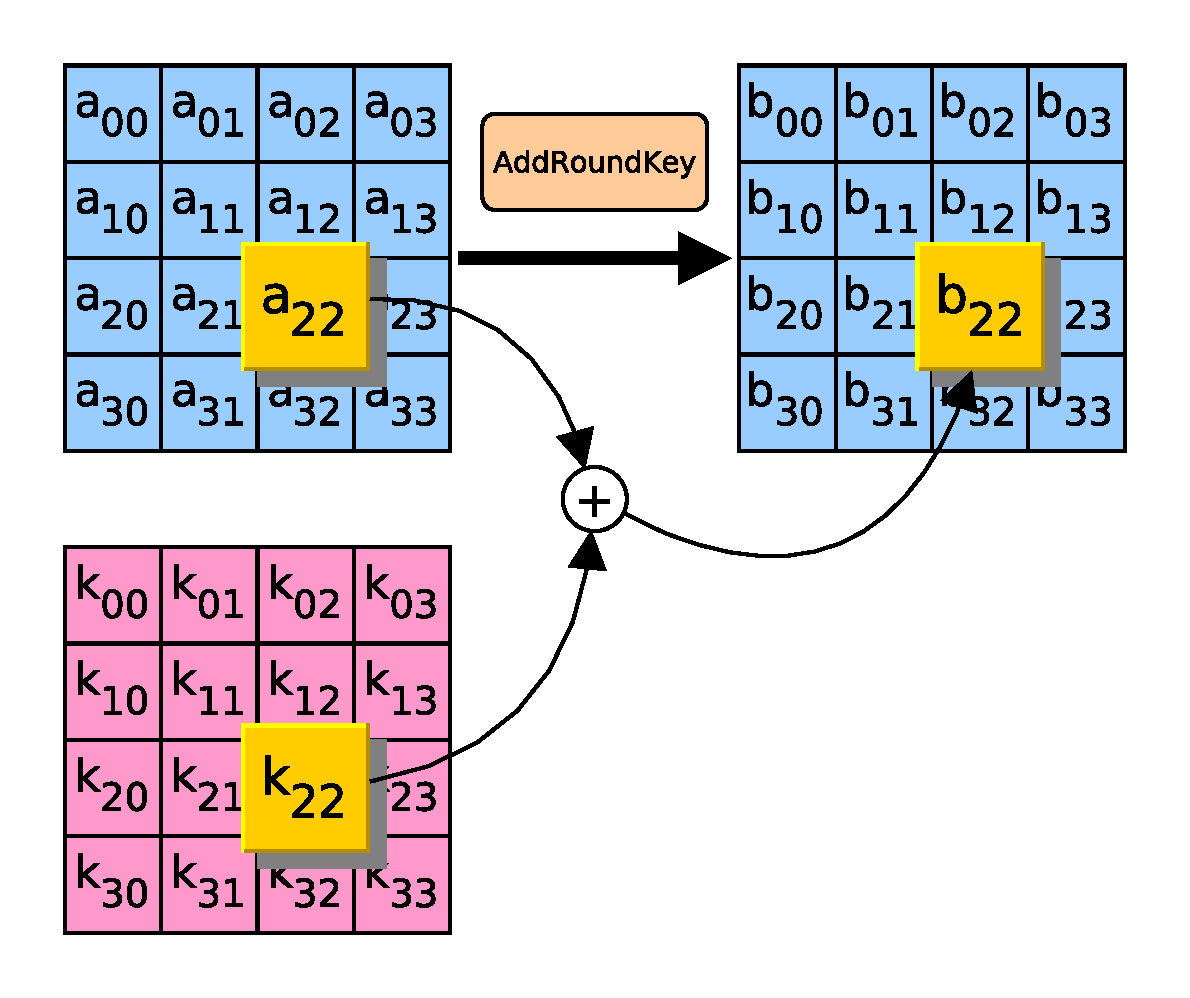
\epsfig{file=addroundkey.eps,width=0.9\columnwidth}
     \caption{A.R.}
     \label{fig-addroundkey}
  \end{minipage}
  \begin{minipage}[t]{0.4\linewidth}
     \centering
     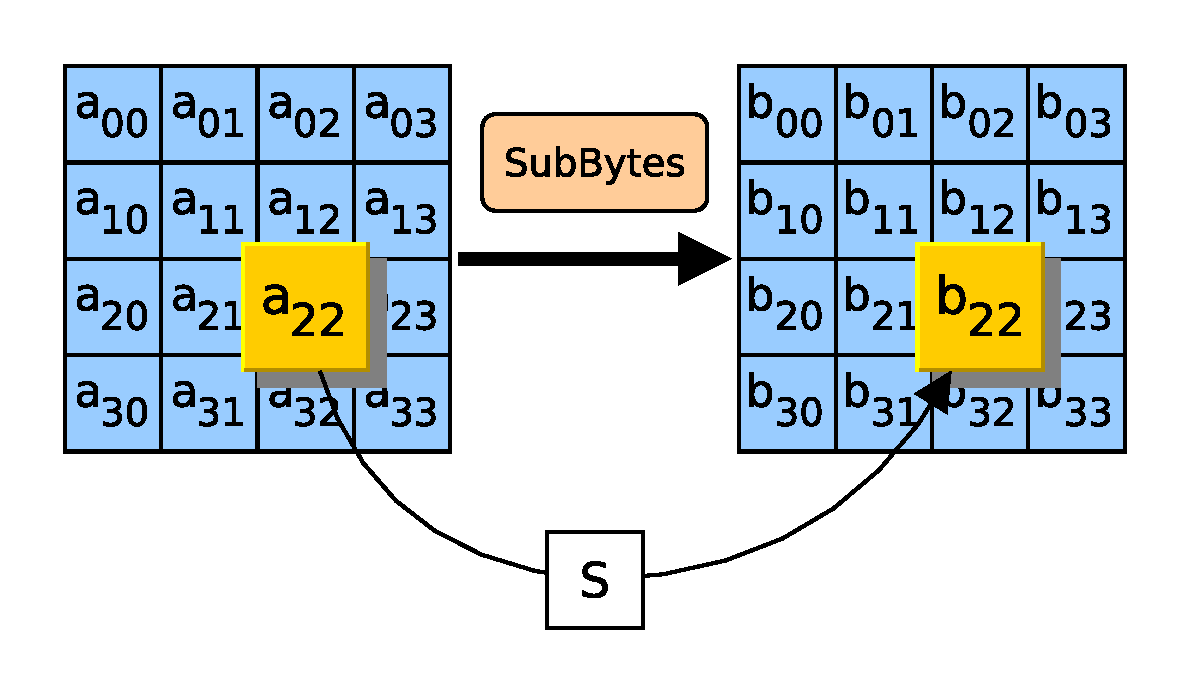
\epsfig{file=subbytes.eps,width=0.9\columnwidth}
     \caption{S.B.}
     \label{fig-subbytes}
  \end{minipage}
  \begin{minipage}[t]{0.4\linewidth}
     \centering
     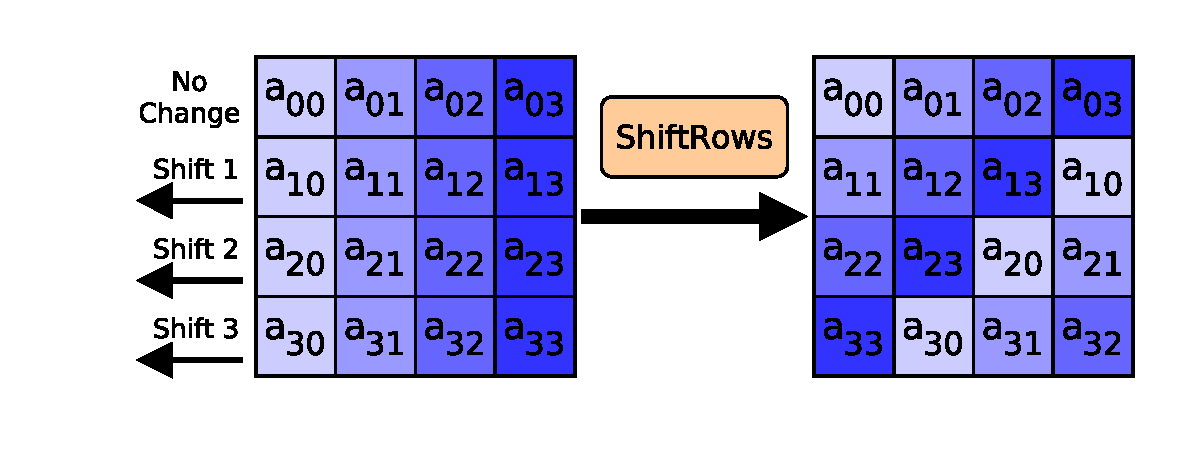
\epsfig{file=shiftrows.eps,width=0.9\columnwidth}
     \caption{S.R.}
     \label{fig-shiftrows}
  \end{minipage}
  \begin{minipage}[t]{0.4\linewidth}
     \centering
     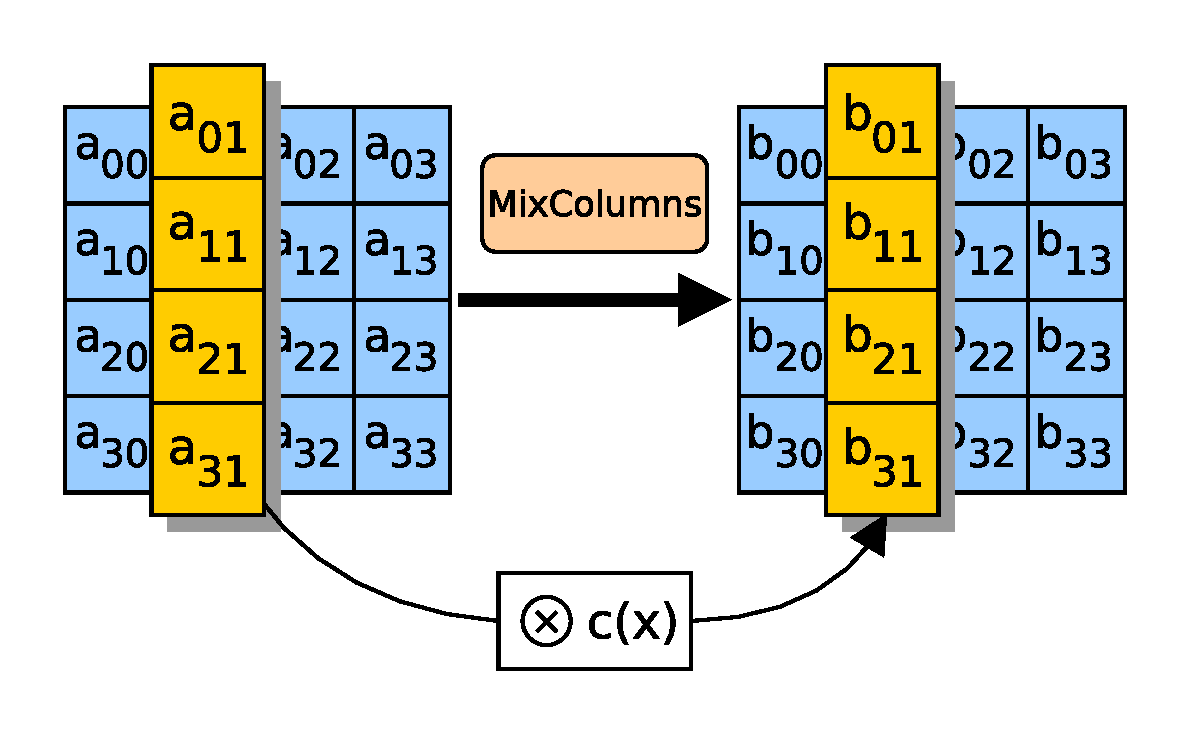
\epsfig{file=mixcolumns.eps,width=0.9\columnwidth}
     \caption{M.C.}
     \label{fig-mixcolumns}
  \end{minipage}
\end{figure}
\subsubsection{Implementatin of AES}
Fig \ref{fig-aesdatapath} shows the dataflow of AES with 128-bit key. We should be aware of that the size of input text is 128-bit, however SubBytes operation gets 8-bit data flows into the S-box each time. So, there comes different configurations of the S-box number. For example, we can use only 1 S-box and do 16 times of SubBytes operations, or use 4 S-box and do just 4 times of SubBytes operations. Same configurations were found in the MixColumns operation.
\begin{figure}[hbpt]
  \centering
  %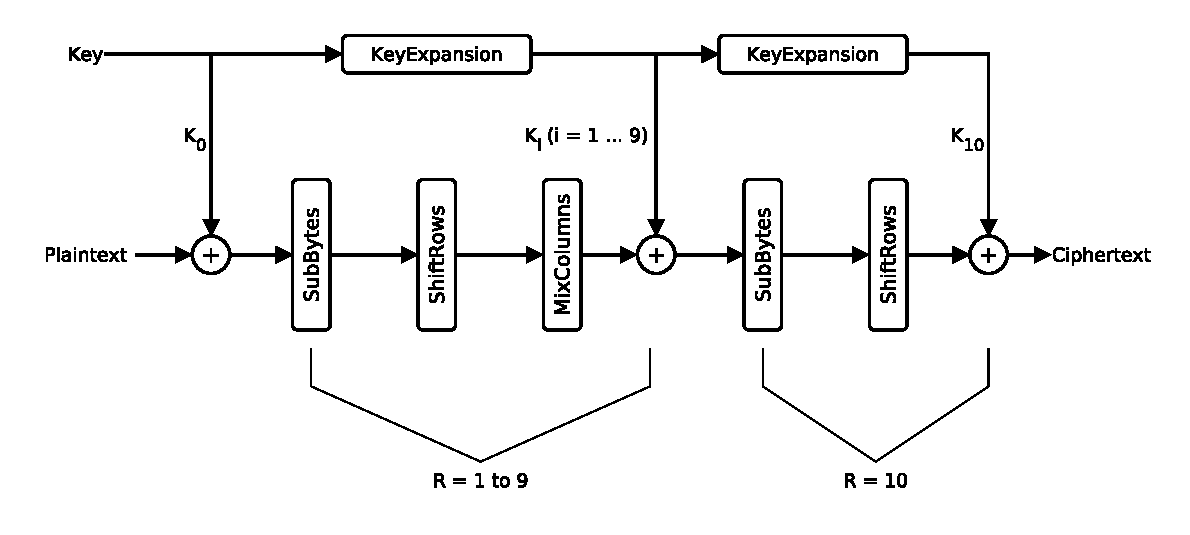
\includegraphics[width=0.1\columnwidth]{DataPathForAES}
  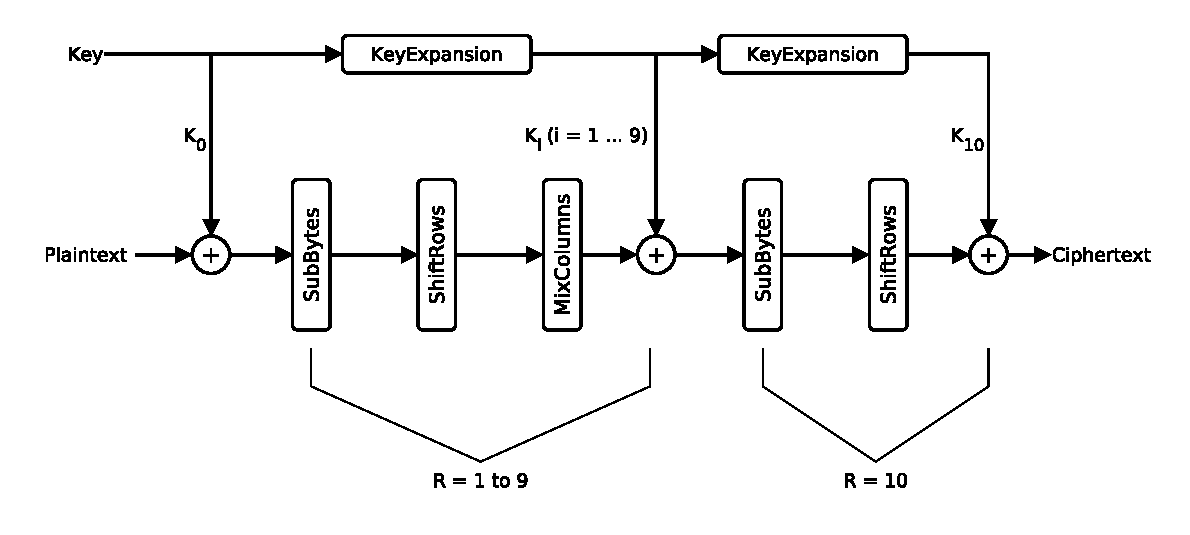
\epsfig{file=DataPathForAES.eps,width=\columnwidth}
  \caption{AES Data Flow}
  \label{fig-aesdatapath}
\end{figure}
\begin{Verbatim}[commandchars=\\\{\}]
always @(posedge clk)
begin   
  if (lddata_i)data <= data_i;
  else if(addkey_i)data <= data_w;
  \Hlight{else if(subbyte_i)map(sbox,data,128,8);}
  else if(mixcolum_i)map(mix,data,128,32);
  else if(shiftrow_i)data <= data_w[127:120], 
                    ..;
end
\end{Verbatim}
%
Where, $sbox$ and $mix$ are two sub-modules, signals $sbox\_i$ and $mixcolumns\_i$ control the invoking of these two sub-modules. Designers don't have to concern the details of the invoke process, such as how $data$ connects with the sub-module, how $data$ flows into sub-module in order. Furthermore, designers can choose the number of sub-modules instances during the compiling process. For different configure choice, the compiler modifies the controller to issue correct control signals in each cycle, as know as  module schedule.

If designers want these configurations without SV+ language constructs, they must write different codes. The following code snippets are just the data transfer part, more codes are needed for module instantiation and $sbox$ input selection.
\begin{Verbatim}[commandchars=\\\{\}]
   Using 1 sbox:           Using 2 sbox:
1. \Vlight{if(subbyte_i)begin     |if(subbyte_i) begin}
2. \Vlight{ data[127:120]<=sbox_o;| data[127:120]<=sbox_o1;}
3. \Vlight{end                    | data[119:112]<=sbox_o0;}
4.                        \Vlight{|end}    
\end{Verbatim}
\begin{Verbatim}[commandchars=\\\{\}]
   Using 4 sboxes:           Using 8, 16 sboxes:
1. \Vlight{if(subbyte_i) begin      | .....}
2. \Vlight{ data[127:120]<=sbox_o3;}
3. \Vlight{ data[119:112]<=sbox_o2;}
4. \Vlight{ data[111:104]<=sbox_o1;}
5. \Vlight{ data[103:96]<=sbox_o0;}
6. \Vlight{end}
\end{Verbatim}
\section{Conclusion}
We implement a novel sequence-based dependency parsing
framework which takes advantage of high order features 
in parsing history. 
%We can also adapt beam search to this framework so as to
%relax the strictly greedy nature. Vine pruning\cite{rush2012vine} could
%be incorporated to speed up the parsing.
More importantly, we discovered that the parsing accuracy is very sensitive to
the quality of parsing sequence. Future work can be focused on
developing better sequence predictors that outperform Malt action classifier.
Furthermore, we use two sets of features for sequence predictor and
head mapper right now. A unified set of features between these two components
are worth exploring.
%Besides, better sequence predicting method and unified feature
%representation of two components are worth exploring.
%
%Though we currently get a not bad result,
%the sequence predictor still needs more exploration.
%According to our experiment, slightly changes
%on the sequence can lead to a fatal decline on accuracy. Ensuring the match degree of training sequence and testing
%sequence demands a high quality of sequence predictor.
%
%Further, the features in our current implementation are not expanded and well tuned yet  and we are free to define high order features to make use of parsing history. Our framework is flexible to merge other technics to enhance the performance. Introducing beam could make up for our greedy decoder and improve our accuracy. Vine pruning\cite{rush2012vine} could speed up parsing process. Besides, better sequence predicting method and unified feature representation of two components are worth exploring.

\bibliographystyle{abbrv}
\bibliography{chip}
\end{document}
